%-----------------------------------------------------------------------------------------------------------------
% File: __TPbckwrd.tex
%
% Code for the backwards writing example for the package texpower.sty.
% 
% This file is input by others. Don't compile it separately.
%
%-----------------------------------------------------------------------------------------------------------------
% Autor: Stephan Lehmke <Stephan.Lehmke@cs.uni-dortmund.de>
%
% v0.0.1 Mar 20, 2000: First version for the pre-alpha release of TeXPower.
%
% v0.0.2 Apr 26, 2000: Some small changes in preparation of the update to TeXpower v0.0.7.
%
% v0.0.3 May 18, 2000: New file name to avoid confusion with ``background''.
%

  %-----------------------------------------------------------------------------------------------------------------
  %
  \makeslidetitle{\macroname{stepwise} Example: Writing Backwards}\label{Sec:ExBackwards}
  %
  % The following example doesn't really demonstrate a useful application. Its purpose is twofold:
  % a) Show how the functionality of \stepwise can be extended by the user by referring to the macros provided by the
  %    package.
  % b) Show that \steps can appear in any order, and can be made to appear simultaneously in several places (and mention
  %    the problems this raises). 

  % We define a new macro \backstep which will call \step, but the steps will be executed in _reverse_ order.
  % This is achieved as follows:
  % * We refer to the counter totalsteps, which gives the total number of steps occurring in this argument of
  %   \stepwise.
  % * From this, we subtract the value of the counter stepcommand, which gives the number of this \step command (in the
  %   order of appearance). 
  % * The result is compared with the counter step, which gives the number of the current step.
  % (the default for `triggering' a \step is the condition \value{step}=\value{stepcommand})
  %
  % Note that if the ifthen Package would support this syntax, we could use the bracketed optional argument of \step (as
  % in the previous example), defining \backstep like this:
  % 
  % \newcommand{\backstep}{\step[\value{totalsteps}-\value{stepcommand}+1=\value{step}]}
  %
  % As \ifthenelse doesn't offer this syntax, we have to calculate \value{totalsteps}-\value{stepcommand}+1 in a separate
  % counter. This doesn't fit the intended use of \step's optional argument. But hey, there is another syntax ;-)
  % If the optional argument is specified with braces (...), then it can contain an arbitrary test which takes two
  % arguments and selects the first if it succeeds and the second if it fails. We use this variant here.
  %
  \newcounter{reversestepno}%
  \newcommand{\backstep}{\step(\setcounter{reversestepno}{\value{totalsteps}-\value{stepcommand}+1}\ifthenelse{\value{step}=\value{reversestepno}})}%
  % 
  % We use the custom command \parstepwise which not only wraps the whole argument of \stepwise into a minipage (because
  % otherwise vertical spacing goes haywire, don't ask me why), but also gives substance to steps.
  %
  % If the following \stepwise command would only contain the calls to \backstep, everything would be fine.
  % But we _had_ to add something else....
  % In the second part of this application of \stepwise, several steps are executed simultaneously with those executed
  % backwards in the first part. This means the value of the counter totalsteps is 14, i.e. the calls to \backstep
  % correspond to steps 8...14. To remedy this, we decree that the first step performed shall be number 7, by setting
  % the counter firststep accordingly in the optional argument of \stepwise.
  % 
  \parstepwise[\setcounter{firststep}{\value{totalsteps}/2+\value{firststep}}]
  {%
    \begin{quote}
      \Huge 
      \backstep{Is} \backstep{now} \backstep{it}
      \backstep{backwards} \backstep{write} \backstep{to}
      \backstep{possible\,!}
      
      \bigskip
        
      % By determining explicitly the times at which the following steps are executed, we make them appear
      % simultaneously with the preceding flock of \backsteps. As we have set the counter firststep to 7, we start
      % counting with 8.
      %
      \step[\value{step}=8]{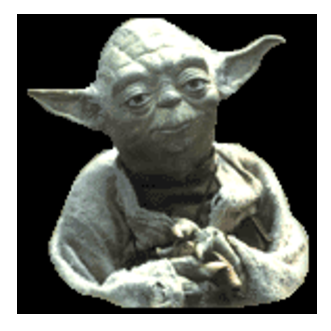
\includegraphics[width=2cm]{yoda}}
      \step[\value{step}=9]{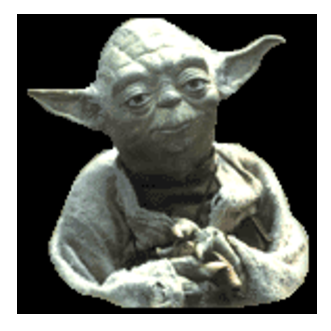
\includegraphics[width=2cm]{yoda}}
      \step[\value{step}=10]{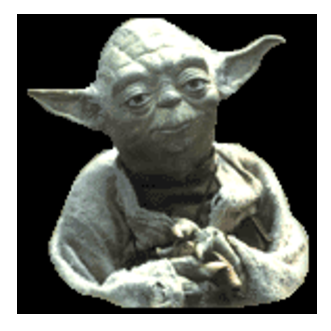
\includegraphics[width=2cm]{yoda}}
      \step[\value{step}=11]{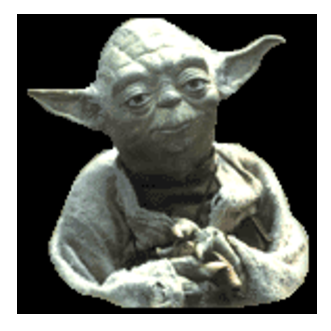
\includegraphics[width=2cm]{yoda}}
      \step[\value{step}=12]{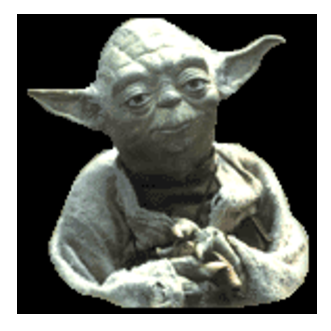
\includegraphics[width=2cm]{yoda}}
      \step[\value{step}=13]{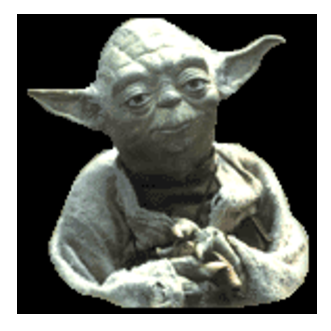
\includegraphics[width=2cm]{yoda}}
      \step[\value{step}=14]{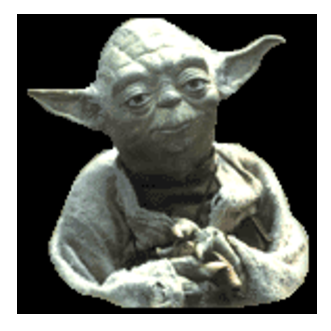
\includegraphics[width=2cm]{yoda}}%
    \end{quote}
    }%


%%% Local Variables: 
%%% mode: latex
%%% TeX-master: "bckwrdexample"
%%% End: 
